\documentclass[12pt]{report}

\renewcommand{\thesection}{\arabic{section}}

\usepackage[letterpaper, dvips, margin=1in, tmargin=1.25in, bmargin=0.75in, head=0.75in, foot=0.25in]{geometry}
\usepackage{fancyhdr}
\usepackage{graphicx}
\usepackage{palatino}
\usepackage{longtable}
\usepackage{float}
\usepackage{calc}
\usepackage[colorlinks=true, bookmarks=true]{hyperref}

\pagestyle{fancy}
\fancyhead[L]{Modeller}
\fancyhead[C]{
\includegraphics[width=1.5in]{logo_black.png}}
\fancyhead[R]{Version 1.01} % Change also in setup.py, cbmodel.py
\fancyfoot{}
\fancyfoot[C]{\thepage}
\renewcommand{\headrulewidth}{0.5pt}
\renewcommand{\footrulewidth}{0.5pt}

\begin{document}

\floatstyle{plain}

\title{
\includegraphics[width=2.5in]{logo_black.png}\\\vspace{0.5in}Modeller\\Version 1.00}
\author{Seven:Twelve Engineering LLC}
\date{}
\maketitle

\clearpage

\section{Introduction}

Welcome to the Crossbeams Modeller!  This manual shows you how to
assemble virtual Crossbeams designs and generate instructions on your
computer.

\section{Installation}

Follow the directions in the {\tt README} file that came with this
distribution.

\subsection{Running}

If you installed from a binary distribution, shortcuts to cbmodel
should already be available on your desktop.  You may also run cbmodel
from the command line with {\tt cbmodel} or {\tt ./cbmodel} from
within the cbmodel install directory.

The Crossbeams Modeller allows the following command-line arguments:

\begin{center}
\begin{tabular}{llp{3in}}
Short Form & Long Form & Description\\
\hline
{\tt -h} & {\tt --help} & Displays the possible options and exits\\
{\tt -i} & {\tt --indirect} & Forces indirect (software-driven, not graphics-card driven) drawing.  Slow but useful for generating instruction sets that go off-screen on some graphics cards.\\
{\tt -p} & {\tt --printkeys} & Displays the key code of the key pressed in the \emph{Status Bar}.  Useful for creating custom key shortcuts.\\
{\tt -a} & {\tt --alpha} & Uses alpha-numeric keys for navigation instead of the numeric keypad.
\end{tabular}
\end{center}

\section{The Main Screen}

% To screen capture a program, type xwd -out screen.xwd.  (Check the
% xwd man page for more options.)  Then, click on the window you want
% captured, and it will be saved to a file called screen.xwd.  Open
% the image in gimp, and you can edit it.
% In gimp, I annotated with:
% 12 pixel rounded strokes for box selection
% 8 pixel rounded strokes for line selection
% 24 point Sans-Bold for fonts
% I also used a graphics include width for 200dpi

\begin{figure}[h]
\begin{center}
%\includegraphics[width=\textwidth]{manual_main_screen.png}
\includegraphics[width=5.1in]{doc_images/manual_main_screen.png}
\caption{Crossbeams Modeller Main Screen}
\label{MainScreen}
\end{center}
\end{figure}

The Crossbeams Modeller shows four main parts (see Figure
\ref{MainScreen}): a menu bar, an editing window, a piece selector, and
a status bar.

\begin{list}{}{}
  \item \emph{Menu Bar:} Allows pull-down menu commands.
  \item \emph{Editing Window:} Shows the model that is being created (drawn in white) and the current piece that is being added (drawn in green).
  \item \emph{Piece Selector:} Allows you to change the current piece.
  \item \emph{Status Bar:} Displays status messages at the left and refresh time at the right.
\end{list}

\section{Building}

\begin{figure}[h]
\begin{center}
%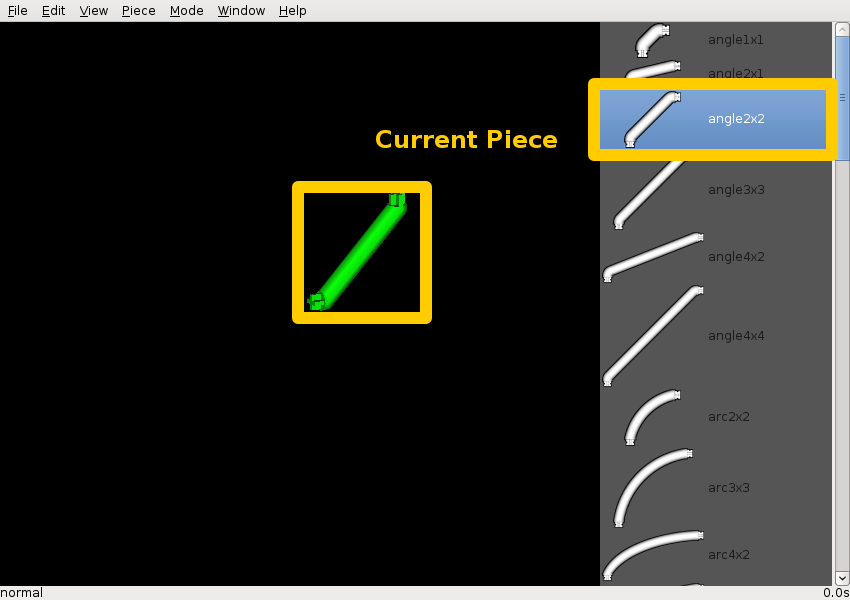
\includegraphics[width=\textwidth]{doc_images/manual_current_piece.png}
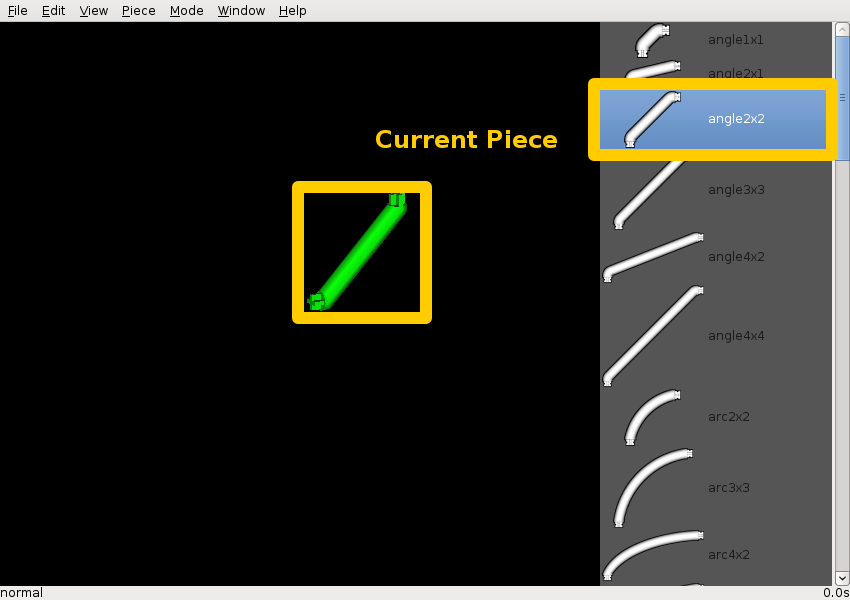
\includegraphics[width=4.0in]{doc_images/manual_current_piece.png}
\caption{Choosing a Piece}
\label{CurrentPiece}
\end{center}
\end{figure}

Ready to begin?  To begin connecting pieces, choose a piece from the
piece selector by clicking on it.  That piece (the \emph{current
  piece}) will be green in the editing window (Figure
\ref{CurrentPiece}).  When starting a new design, the first piece is
    {\tt attached} to an invisible cross-hair (like a `+' sign) in the
    center of the editing window.  To {\tt attach} that initial piece
    to a different part of the cross-hair, click a little left, up,
    down, or right of center.

\begin{figure}[h]
\begin{center}
%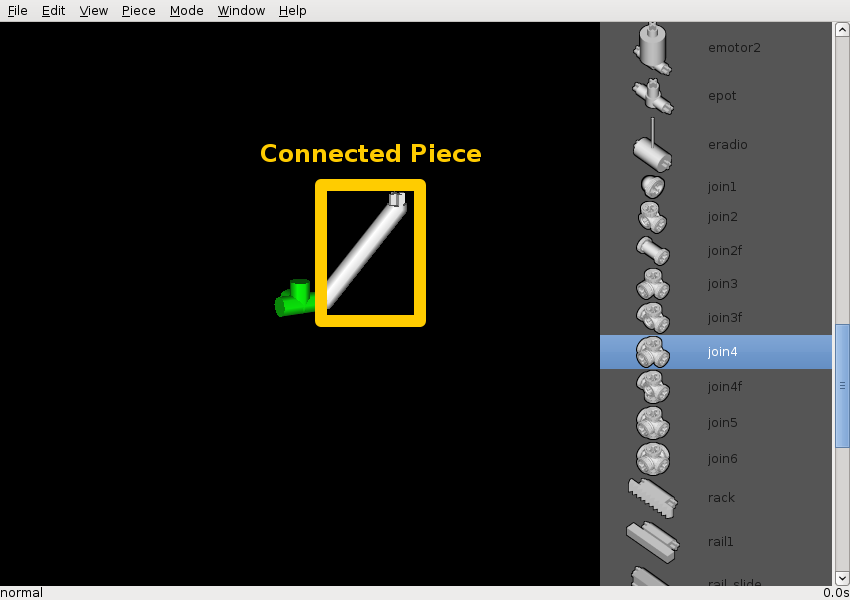
\includegraphics[width=\textwidth]{doc_images/manual_connected_piece.png}
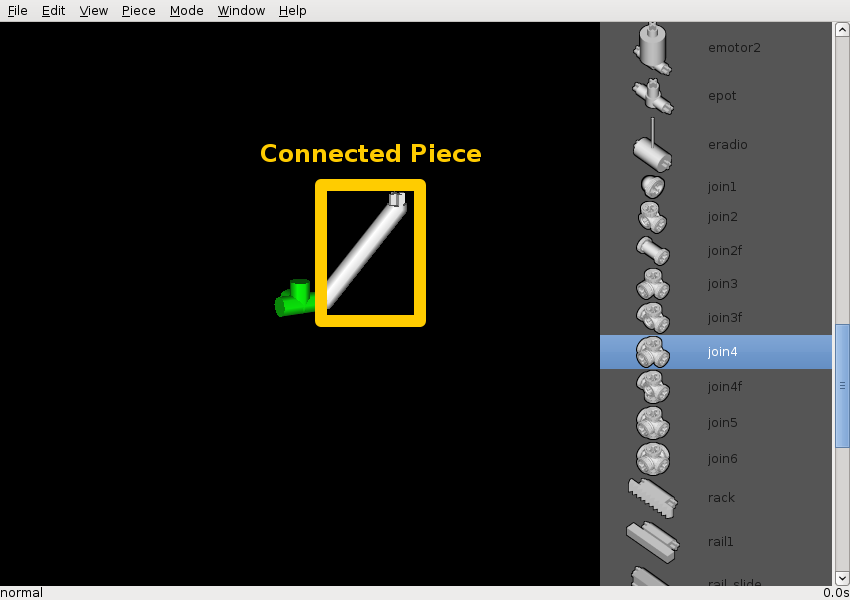
\includegraphics[width=4.0in]{doc_images/manual_connected_piece.png}
\caption{Connecting a Piece}
\label{ConnectedPiece}
\end{center}
\end{figure}

When you have the piece you want, press {\tt c}\footnote{Nearly all
  key commands have pull-down menu equivalents.  The key commands may
  be customized.} (for connect) to connect it.  You've just
established the first piece of your design (or \emph{model}).  Notice
it is no longer green but white (Figure \ref{ConnectedPiece}).  A new
current piece (green) appears automatically.

Often, the automatic piece is not the next one you want to connect.
Choose a different piece by clicking on it in the piece selector.

\begin{figure}[h]
\begin{center}
%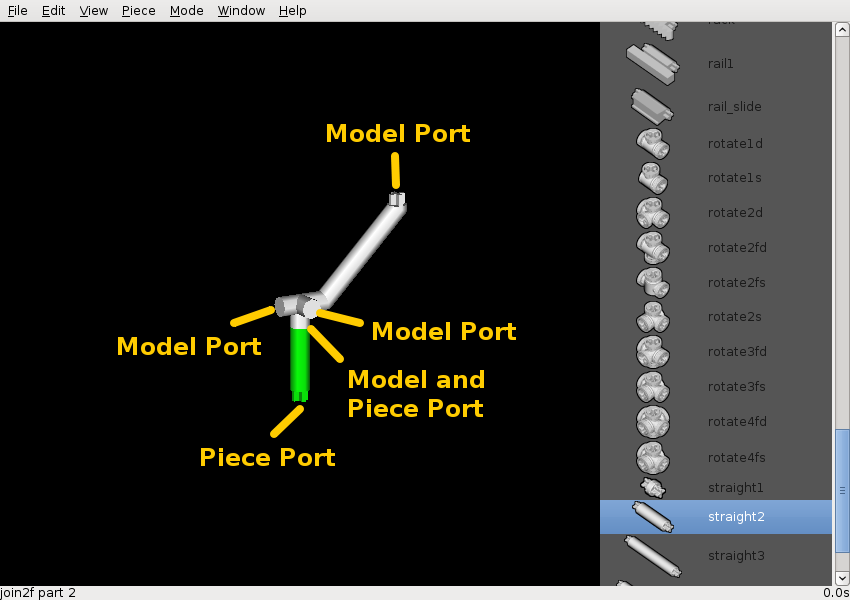
\includegraphics[width=\textwidth]{doc_images/manual_ports.png}
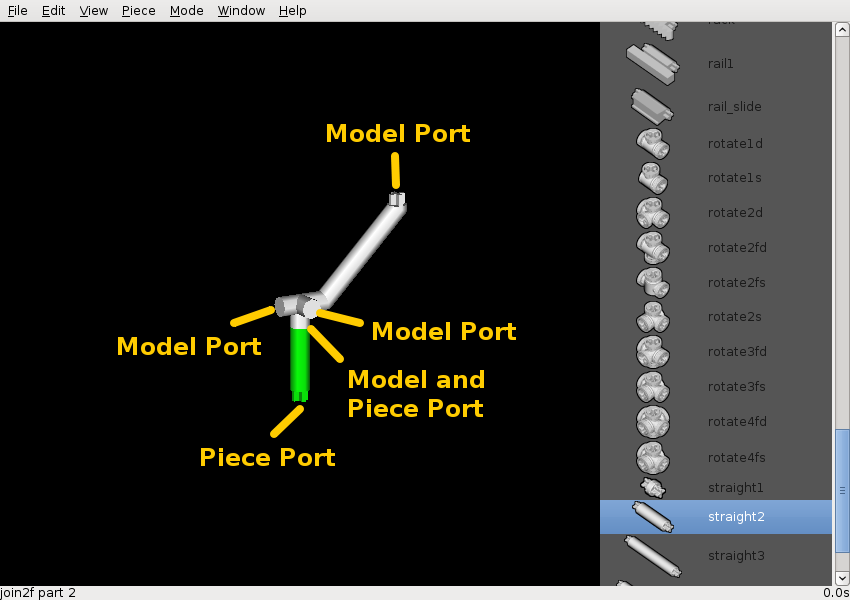
\includegraphics[width=4.0in]{doc_images/manual_ports.png}
\caption{Ports}
\label{Ports}
\end{center}
\end{figure}

Every piece has at least one place to connect to other pieces.  These
connection points are called \emph{piece ports}.  Likewise, every
model has zero or more unconnected ports (Figure \ref{Ports}) called
\emph{model ports}.  Left-click on the model port where you want the
piece to connect.  You'll see the current piece move to the model
port.

You can choose a different piece port to connect to the model port by
pressing {\tt p} (for port).

You can rotate the piece in $90 ^\circ$ increments by pressing {\tt f}
(for flip).

Once the piece is where you want it, press {\tt c} to connect.  The
piece changes from green to white when it is connected, and a new
current piece (in green) attaches itself to another model port.

The Crossbeams Modeller knows joints can only be connected to beams
and beams can only be connected to joints.  (The main pieces are
either \emph{beams} or \emph{joints}.)  After you connect a piece, the
system will automatically attach the most recent beam or joint to a
new model port.

Continue building in the same way: 

\begin{enumerate}

  \item Click on the current piece you want (in the piece selector).
  \item Left-click on the model port where you want the piece to connect.
  \item Choose the correct piece port by pressing {\tt p}.
  \item Choose the correct piece rotation by pressing {\tt f}.
  \item Press {\tt c} to connect.

\end{enumerate}

\subsection{Definitions}
\begin{list}{}{}
  \item \emph{Model:} the total design being built and displayed.
  \item \emph{Current piece:} the piece which is currently selected
    (but not yet connected).  The current piece is always in green.
  \item \emph{Piece port:} the part of the piece which connects with other
    pieces.
  \item \emph{Model port:} an unconnected port in the model.
\end{list}

\subsection{Building Command Summary}
\begin{list}{}{}
  \item To \textbf{select a different piece port}, press {\tt p}.
  \item To \textbf{rotate the current piece}, press {\tt f}.
  \item To \textbf{connect the current piece to the model}, press {\tt c}.
\end{list}

\section{Navigating}

Both keyboard and mouse can control how you view your model, allowing
you to ``move around'' (navigate) in the editing window by panning,
orbiting and zooming.

\subsection{By Keyboard}

To navigate your view using the keyboard, use the following
keys (remember to use the \textbf{numeric keypad} (NumPad)):

\begin{center}
\begin{tabular}{llll}
NumPad Key & Action & NumPad Key & Action\\
\hline
{\tt 8} & orbit up & {\tt Shift 8} & pan up\\
{\tt 2} & orbit down & {\tt Shift 2} & pan down\\
{\tt 4} & orbit left & {\tt Shift 4} & pan left\\
{\tt 6} & orbit right & {\tt Shift 6} & pan right\\
{\tt *} & rotate clockwise & {\tt +} & zoom in\\
{\tt /} & rotate counterclockwise & {\tt -} & zoom out\\
{\tt 7} & top view & {\tt Shift 7} & bottom view\\
{\tt 1} & front view & {\tt Shift 1} & back view\\
{\tt 3} & right-side view & {\tt Shift 3} &left-side view\\
\label{KeyTable}
\end{tabular}
\end{center}

The direction is from your perspective.  For example, \emph{orbit up}
means you \emph{orbit up} while the model remains stationary.

What if you don't have a NumPad?  You may start the Crossbeams
Modeller with the {\tt --alpha} option to force alpha (non-NumPad)
keys.  Alternatively, you may select alpha keys with {\tt Options -
  Navigation with Alphas}.  In the latter case, you must exit and
restart the Crossbeams Modeller before the new keys are active.  Then,
use the following keys to navigate:

\begin{center}
\begin{tabular}{llll}
NumPad Key & Action & Key & Action\\
\hline
{\tt i} & orbit up & {\tt Shift i} & pan up\\
{\tt ,} & orbit down & {\tt Shift ,} & pan down\\
{\tt j} & orbit left & {\tt Shift j} & pan left\\
{\tt l} & orbit right & {\tt Shift l} & pan right\\
{\tt 8} & rotate clockwise & {\tt +} & zoom in\\
{\tt 9} & rotate counterclockwise & {\tt -} & zoom out\\
{\tt u} & top view & {\tt Shift u} & bottom view\\
{\tt m} & front view & {\tt Shift m} & back view\\
{\tt .} & right-side view & {\tt Shift .} &left-side view\\
\label{AlternateKeyTable}
\end{tabular}
\end{center}

The rest of the manual assumes you use NumPad.  If you don't,
substitute the appropriate key from the table above.

\subsection{By Mouse}

You can also orbit or pan your view by using the mouse.

\begin{list}{}{}
  \item To \textbf{orbit}: move the mouse while holding down on the
    middle mouse button
  \item To \textbf{pan}: press {\tt Shift} and move the mouse while
    holding down on the middle mouse button.
\end{list}

On computers without a middle mouse button, holding down {\tt Control}
while holding down the left mouse button substitutes as a middle mouse
button.

\section{Editing}

\subsection{Undo/Redo}

You can undo the last model change with {\tt Edit - Undo} or {\tt
  Control z}.  You can redo the last model change with {\tt Edit -
  Redo} or {\tt Control y}.

\subsection{Selecting}

\begin{figure}[h]
\begin{center}
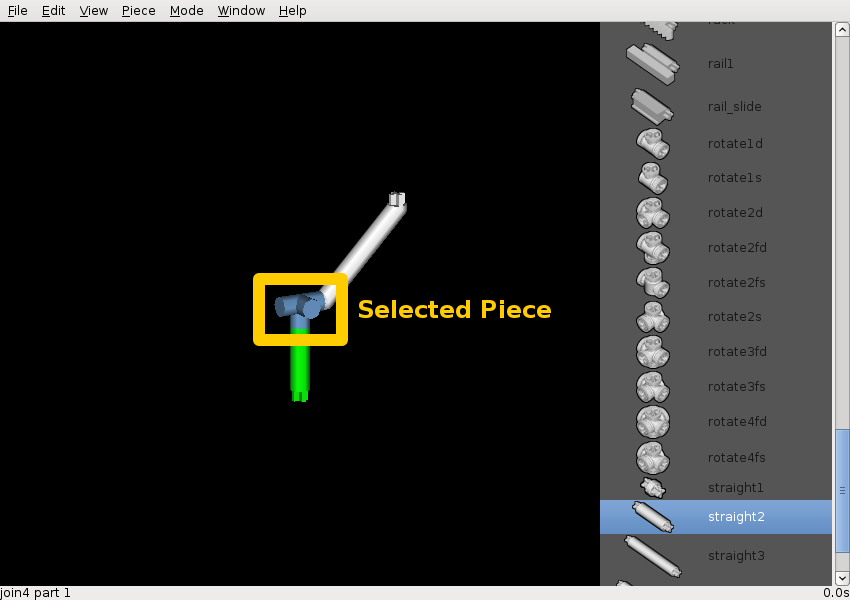
\includegraphics[width=4.0in]{doc_images/manual_selecting.png}
\caption{Selecting Pieces}
\label{Selecting}
\end{center}
\end{figure}

To select a piece, right-click on the center of the piece.  The
selected piece becomes blue.  To select multiple pieces, hold {\tt
  Shift} while right-clicking an unselected piece (Figure
\ref{Selecting}).  Look around your model by navigating to make sure
the selected piece is the one you really want.  (For example, when
other pieces lie exactly behind the piece you want, the Crossbeams
Modeller may choose one of those instead.)

To border-select a group of pieces, press {\tt b} (for box).  Then,
position the mouse at the upper-left corner of the box.  Left-click on
the upper-left corner, drag to the lower-right corner, and release.
Pieces whose centers fall within the border are selected.

To deselect a single piece from multiple pieces, hold {\tt Shift}
while right-clicking a selected piece.  Press {\tt a} (for all) to
deselect all pieces when some are selected.  Press {\tt a} to select
all pieces when none are selected.

To select pieces of a specific type, choose a piece from the piece
selector.  Then use {\tt Edit - Select by Type}.

The status bar displays the number of selected pieces.

\subsection{Configuring}

\begin{figure}[h]
\begin{center}
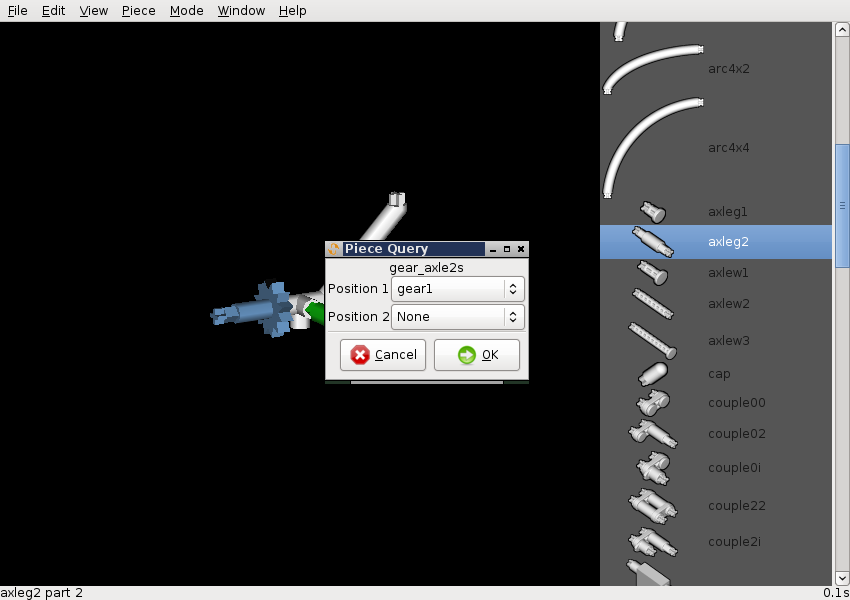
\includegraphics[width=4.0in]{doc_images/manual_configuring.png}
\caption{Configuring a Piece}
\label{Configuring}
\end{center}
\end{figure}

axlews and axlegs can be configured to have various numbers and types
of wheels and gears on them.  Rotating joints can be configured to
have stiffens on them.  To configure a piece, select it, and press
{\tt q} (for query).  A Piece Query window pops up (Figure
\ref{Configuring}).  Configure the piece by choosing the appropriate
pulldowns.  Click {\tt OK} to accept or {\tt Cancel} to cancel.

\subsection{Deleting}

To delete selected pieces, press {\tt x}.

\subsection{Moving}
To move selected pieces, first grab them by pressing {\tt g} (for
grab).  The grabbed pieces follow mouse movement.  To cancel the grab,
right-click the mouse.  To accept and finish the grab, left-click the
mouse.  Grabbed pieces move in half unit increments.

\subsection{Copying}
To copy (duplicate) selected pieces, press {\tt Shift d} (for
duplicate).  \emph{Duplicate} copies the selected pieces, makes the
new (copied) pieces the selected ones, and puts the new pieces in grab
mode.  The copied pieces must be moved for \emph{duplicate} to work.

\subsection{Rotating}
To rotate selected pieces in $90 ^\circ$ increments, position the
mouse at the fulcrum (the point you want the pieces to rotate around),
and press {\tt r} (for rotate).  Move the mouse to rotate.  $0 ^\circ$
is to the right.  To cancel the rotate, right-click the mouse.  To
accept and finish the rotate, left-click the mouse.

\subsection{Mirroring}
To mirror selected pieces, choose a model port to be the fulcrum (the
point you want the mirror image to mirror about).  Position the mouse
at that model port, and press {\tt Control m} (for mirror).

Move the mouse across the plane you want to mirror the pieces in.  To
cancel the mirror, right click the mouse.  To accept and finish the
mirror, left click the mouse.

\subsection{Nuances}

To make the mouse motion more closely approximate what you're seeing,
use orthogonal views (left, right, top, bottom, front, or back) during
grab, duplicate, rotate, and mirror operations.

Grab, duplicate, rotate, and mirror have not been fully debugged for
impossible edits (e.g., overlapping pieces).  Therefore, to avoid
bugs, make sure these edits are physically possible.

Some editing operations sever a model.  The Crossbeams Modeller
treats the severed models as one large model.

\subsection{Fixing}

Impossible edits sometimes corrupt a model.  {\tt Edit - Fix} can fix
some corrupted models.  Unfortunately, it cannot fix all of them.

\subsection{Editing Command Summary}
\begin{list}{}{}
  \item To \textbf{undo the last model change}, press {\tt Control z}.
  \item To \textbf{redo the last model change}, press {\tt Control y}.
  \item To \textbf{select a piece}, right-click on that piece.
  \item To \textbf{select multiple pieces}, press {\tt Shift} and
    right-click on each piece.
  \item To \textbf{border-select a group of pieces}, press {\tt b}.
    Then click-and-drag from upper-left to lower-right.
  \item To \textbf{deselect a piece}, press {\tt Shift} and
    right-click on that piece.
  \item To \textbf{deselect all pieces} when some are selected, press
    {\tt a}.
  \item To \textbf{select all pieces} when none are selected, press
    {\tt a}.
  \item To \textbf{select a single piece type}, use {\tt Edit - Select by Type}.
  \item To \textbf{configure a piece}, press {\tt q} while the axle is selected.
  \item To \textbf{delete selected pieces}, press {\tt x}.
  \item To \textbf{move selected pieces}, press {\tt g}.
  \item To \textbf{copy selected pieces}, press {\tt Shift d}.
  \item To \textbf{rotate selected pieces}, press {\tt r}.
  \item To \textbf{mirror selected pieces}, press {\tt Control m}.
  \item To \textbf{fix a model}, use {\tt Edit - Fix}.
\end{list}

\section{Reporting}

You can view a model's inventory, dimensions, mass, estimated price,
or instruction page count with various {\tt View} menu commands.  Each
one pops up a reporting window.

\subsection{Inventory}

\begin{figure}[h]
\begin{center}
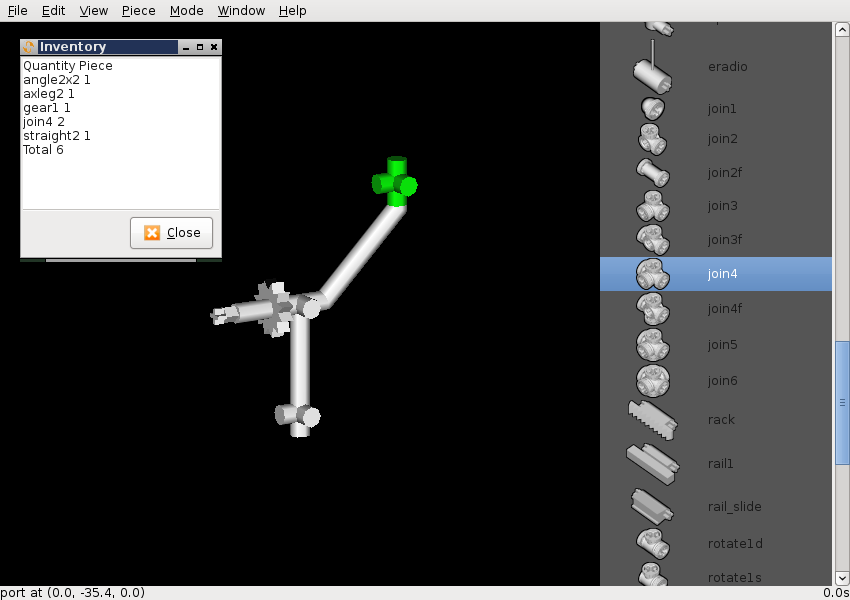
\includegraphics[width=4.0in]{doc_images/manual_inventory.png}
\caption{Reporting the Inventory}
\label{Inventory}
\end{center}
\end{figure}

To view a list of pieces used in your model, use {\tt View -
  Inventory}.

\subsection{Dimensions}

To view the size (dimensions) of your model, use {\tt View -
  Dimensions}.

\subsection{Mass}

To view the mass or weight of your model, use {\tt View - Mass}.

\subsection{Price}

To view an estimated price of your model, neglecting instruction set
and packaging, use {\tt View - Price}.

\subsection{Instruction Page Count}

To view the number of pages in your model's instruction set, use {\tt
  View - Pages}.  You will have zero pages until you add instructions.

\section{Files}

\subsection{Normal File Changes}

{\tt New}, {\tt Open}, {\tt Save}, and {\tt Save As} features can be
found under the File menu.  They operate similarly to most other
programs.  There is no query to save on exit, so make sure you save
often.

Crossbeams Modeller files are saved with a {\tt .cbm} extension.  {\tt
  .cbm} is a text format, so you may view it in a text editor.

\subsection{Saving Snapshots}

Use {\tt File - Save Snapshot} to save a Snapshot (or photo) of your
model in {\tt .png} format.

\subsection{Saving an Inventory}

You may also save a list of all pieces used and their quantity (an
inventory) with {\tt File - Save Inventory}.  The file is saved with
the same name and a {\tt .csv} extension.  {\tt .csv} format is easy
to read.  A comma separates the piece quantity and piece name.

\subsection{Merging Models}

While every file only contains one model, you may merge models from
another file into your current model.  To do so, select the {\tt File
  - Merge} menu option.  Choose the other model's file name, and the
other model will be imported and selected into your current model.  Be
careful.  Usually the other model will overlap your current model
somewhere.  It's best to keep it selected and move it where it doesn't
overlap before deselecting it.

\section{Options}

\begin{figure}[h]
\begin{center}
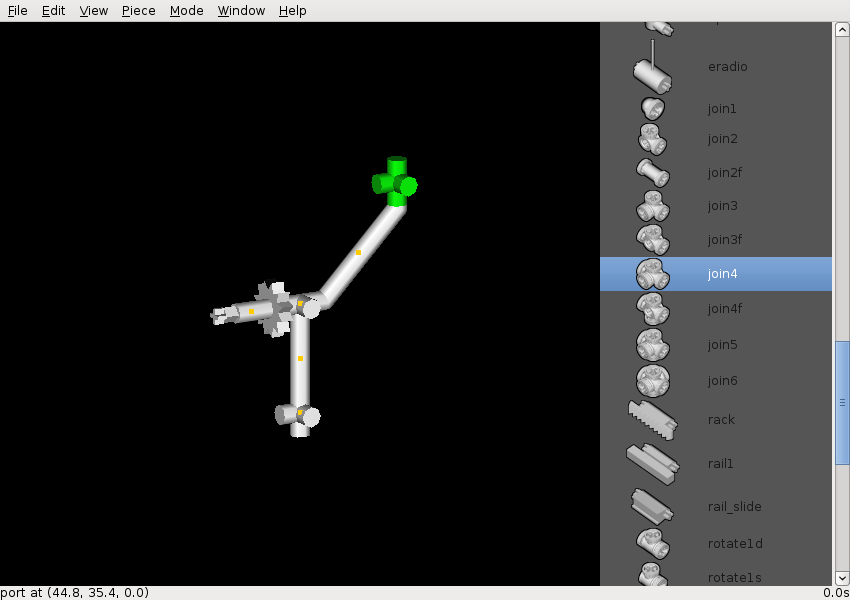
\includegraphics[width=4.0in]{doc_images/manual_centers.png}
\caption{Draw Centers}
\label{DrawCenters}
\end{center}
\end{figure}

\subsection{Detail}

Various levels of detail are allowed in the model drawing.  Solid
detail draws pieces as simple intersecting cylinders.  Render detail
draws the actual piece.  The better the detail, the slower the screen
redraws.  Choose solid detail with {\tt z}.  Choose render detail with
{\tt F12}.  Detail can also be set with {\tt Options - Detail}.

The first time a piece type is rendered takes a long time.  Afterward,
it renders faster.  With a high-end graphics card, render redraws can
be acceptably fast, even while building.

Render detail is currently disabled for public versions of the
Crossbeams Modeller.

\subsection{Window Sizes}

You may resize the window using the window manager.  For instructions,
however, the window must be at fixed sizes.  Select one of the {\tt
  Options - Window Size} menu options to change to a fixed size.

\subsection{Colors}

The Crossbeams Modeller lets you change between Screen (white on
black) and Print (white on white) color schemes.  Select the color
with the {\tt Options - Color} menu options.  To more thickly outline
the parts in black, particularly for white on white, use {\tt Options -
  Draw Outlines}.

\subsection{Draw Centers}

For selection, the piece center is not always clear.  {\tt Options -
  Draw Centers} draws the center point of each piece in a highlighted
color (Figure \ref{DrawCenters}).

\subsection{Navigation with NumPad or Alphas}

You may set your navigation key settings to NumPad or Alphas
(non-NumPad) keys with these two options.  The change doesn't take
effect until you restart.  Be careful: selecting either of these
options writes to your configuration file, overwriting custom key
settings.

\section{Instructions}

\begin{figure}[h]
\begin{center}
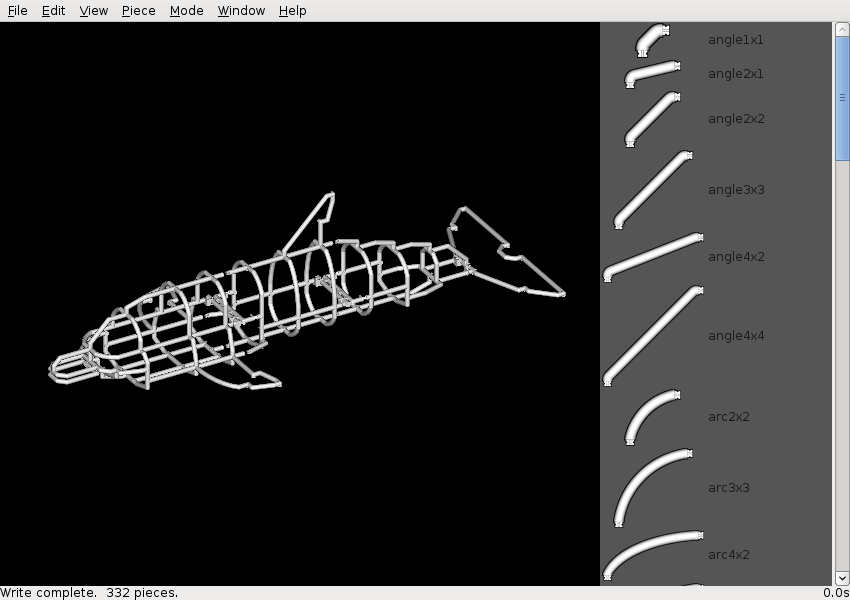
\includegraphics[width=4.0in]{doc_images/manual_instructions_model.png}
\caption{Model Ready for Instructions}
\label{InstructionsModel}
\end{center}
\end{figure}

After you create a fine-looking model (Figure
\ref{InstructionsModel}), you may want to share the idea through an
instruction set.  An instruction set consists of a cover photo of the
model, poses of the model, and a sequence of frames.  The first frame
begins with a blank screen and a few added pieces.  Subsequent frames
add more pieces, until the final frame completes the model.

The Crossbeams Modeller has two main modes: \emph{Modelling} and
\emph{Instructions}.  Before choosing \emph{Instructions} mode,
make sure your model is nearly complete.  \emph{Modelling} changes
often require large \emph{Instructions} changes.

Choose \emph{Instructions} mode with {\tt Mode - Instructions}.  The
{\tt Piece} menu will be replaced by an {\tt Instructions} menu.

\subsection{Cover}

\begin{figure}[h]
\begin{center}
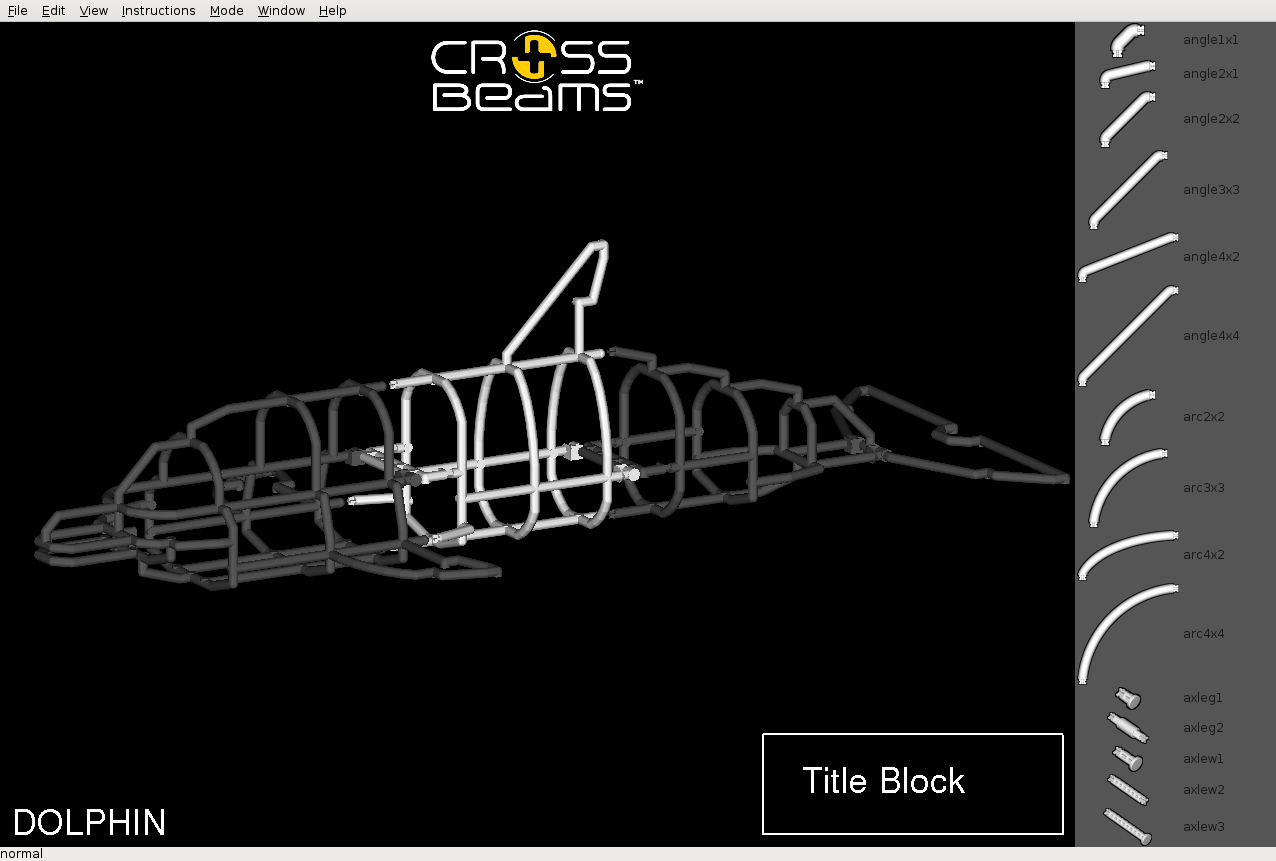
\includegraphics[width=6.38in]{doc_images/manual_instructions_cover.png}
\caption{Cover}
\label{InstructionsCover}
\end{center}
\end{figure}

The first Instructions frame is a full-page cover.  Use the Navigation
keys to position the model for the cover photo.  Use {\tt Instructions
  - Set Title} to set the model's title and author.  Once you are
satisfied with the cover appearance (Figure \ref{InstructionsCover}),
press the {\tt Right} arrow to advance to Frame 1.  If you want to
edit the cover again, simply return to Frame 0 (the cover) with the
{\tt Left} arrow or use {\tt Instructions - Go To Frame}.

\subsection{Poses}

\begin{figure}[h]
\begin{center}
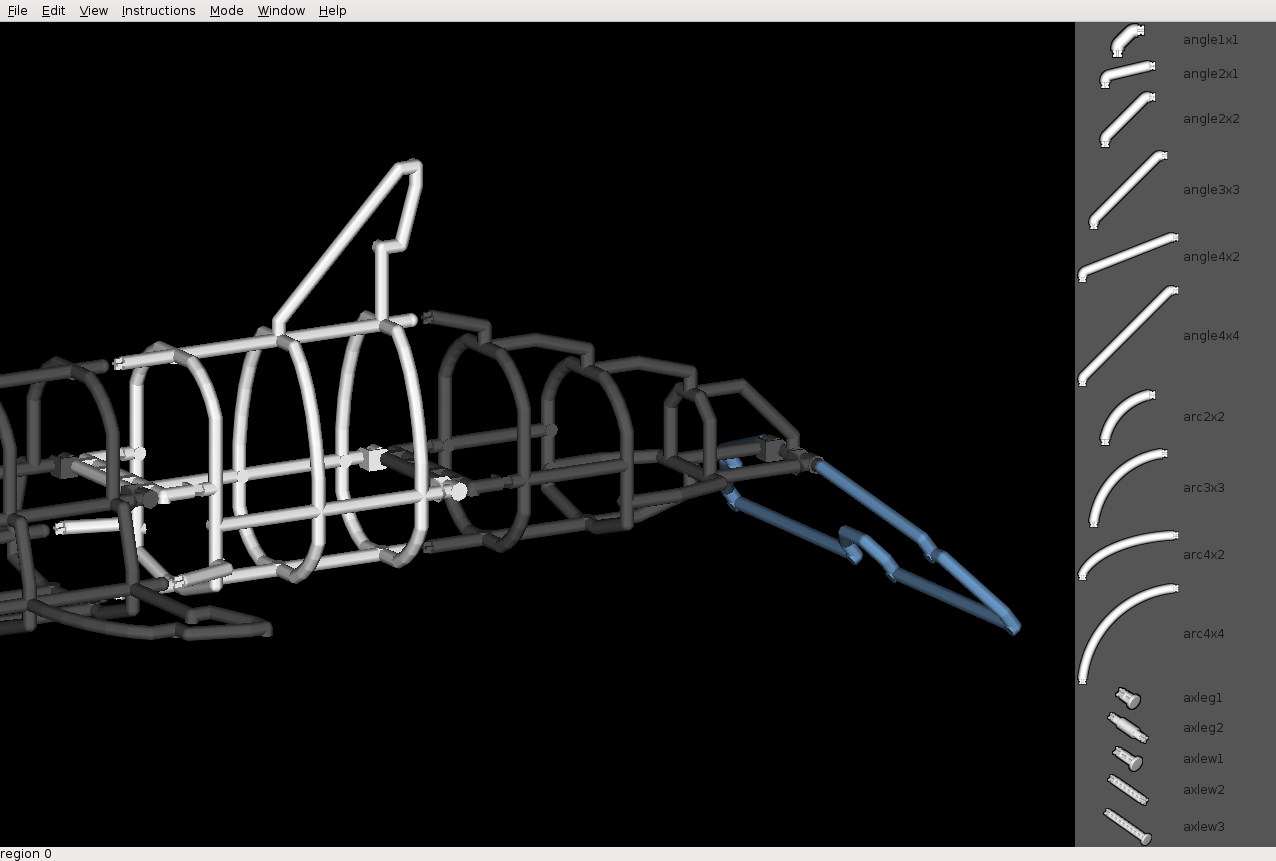
\includegraphics[width=6.38in]{doc_images/manual_instructions_pose.png}
\caption{Pose}
\label{InstructionsPose}
\end{center}
\end{figure}

Before the frames start, you may want to show off various features of
your model: a zoom-in of a geared area, a top view, or a view with
moving regions in a different position, for example.  These are called
{\tt Pose} views, and they come before the frames start.

The cover frame is a Pose view.  To add more Pose views after the
cover, from the cover frame, use {\tt Instructions - Insert After}.
Now, press the {\tt Right} arrow, and you will be in another Pose
view.  Use the Navigation keys to position the model in the new Pose.
Add more Pose views with {\tt Instructions - Insert After} from a Pose
view.

You probably noticed our instruction cover colored parts of the model
white and parts grey.  Models with moving regions can move regions in
a Pose view.  For example, it might be nice to Pose an elephant's
moving trunk, an eagle's flapping wings, a car's opening door, or, in
this case, a dolphin's bending body.  The modeller must always have
one fixed region displayed in white.  Moving regions are displayed in
grey.  Select a moving region by right-clicking at the center of a
moving region.  (The {\tt Options - Draw Centers} option is helpful for
finding the center of a region.)  The region to be moved appears in
blue.  Now, position the mouse at the fulcrum and press {\tt r} (for
rotate).  Move the mouse at various angles from the fulcrum to rotate.
To cancel the rotate, right-click.  To accept and finish the rotate,
left-click.

Sometimes, the model will get messed up with a series of cascaded
region rotates.  The region can be restored to its original position
by pressing {\tt 0} while rotating it.

The fixed region can change by choosing {\tt Edit - Set Selected to
  Fixed}.

\subsection{Frames}

\begin{figure}[h]
\begin{center}
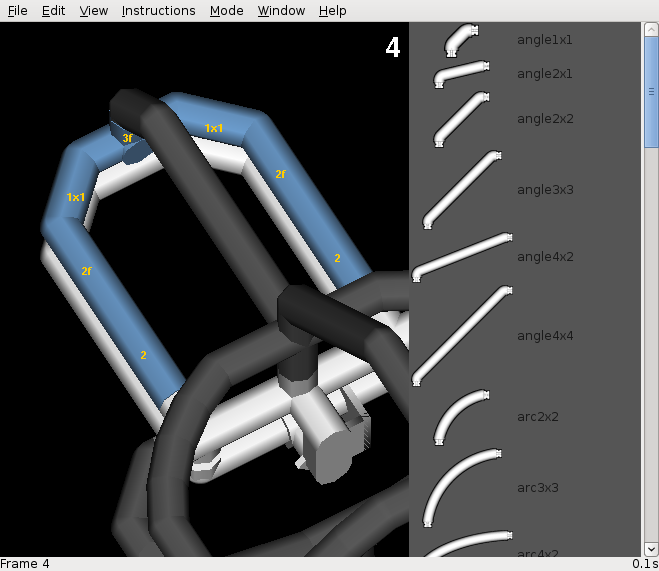
\includegraphics[width=3.29in]{doc_images/manual_instructions_frame1.png}
\caption{Frame}
\label{InstructionsFrame}
\end{center}
\end{figure}

In Frame 1, you'll see an entirely grey version of your model.  Grey
pieces show pieces that haven't yet been added in any instruction
frame.  First, select a frame size from the Window menu.  You may
choose Full, FullR, Quarter, and Half.  By default, the previous
frame's size is used for new frames.  Next, navigate to the region
where you'd like to add pieces.  Pieces added in this frame are shown
blue.  Select the added pieces the same way you select pieces while
modelling.

Pieces added in previous frames are shown white.  You won't see any of
them in Frame 1, but you'll see them in the following frames (Figure
\ref{InstructionsFrame}).

Navigate to get a view that looks good, and advance to the next frame
with the {\tt Right} arrow.  Continue creating instruction frames in
the same way:

\begin{enumerate}

  \item If necessary, choose a new window size.
  \item Navigate to the region where you want to work.
  \item Select the pieces you want to add in the frame.
  \item Navigate to make the view look good.
  \item Store the frame and advance to the next frame by pressing {\tt Right}.

\end{enumerate}

The order up to the advance frame step is unimportant.  For example,
you may change the window size after selection.  Find an order that
works for you.

\subsection{Frame Editing}

Use the {\tt Left} and {\tt Right} arrows to move back and forward
between frames.  Each arrow press stores the displayed frame's state,
so don't change anything as you navigate unless you want it changed.

Use {\tt Instructions - Go To Frame} to move to any frame in the set.
Use Frame 0 to move to the cover.  Use a number equal to or larger
than the number of frames to move to the last frame.

Use {\tt Instructions - Insert Before} and {\tt Instructions - Insert
  After} to insert a frame before or after the current frame.  Use
{\tt Instructions - Delete Frame} to delete the current frame.

\subsection{Cross Hair}

\begin{figure}[H]
\begin{center}
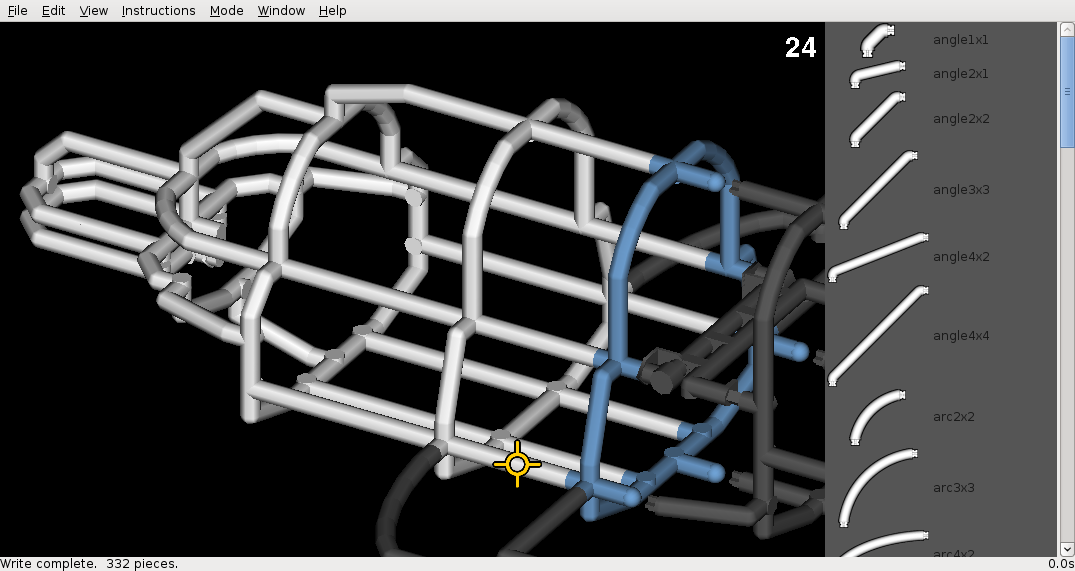
\includegraphics[width=5.38in]{doc_images/manual_instructions_xhair.png}
\caption{Cross Hair}
\label{InstructionsXhair}
\end{center}
\end{figure}

When you navigate far between two frames, it's not always obvious
where you are.  You may use the cross hair icon to help.  Use {\tt
  Instructions - Show Cross Hair} to display a cross hair icon in your
current frame.  Drag the icon with the left mouse button over the next
frame's center piece (Figure \ref{InstructionsXhair}).

\subsection{Hide/Unhide Parts}

It can be difficult to select inner pieces in extremely dense models.
You may hide exterior pieces to more easily see innexor pieces.
Select the pieces you want to hide.  Then, use {\tt Edit - Hide
  Selected} pieces to hide them.  Make sure you later reveal them with
{\tt Edit - Unhide} so your instructions include all pieces.  The
status bar displays the number of hidden pieces.

\subsection{Mirror}

\begin{figure}[H]
\begin{center}
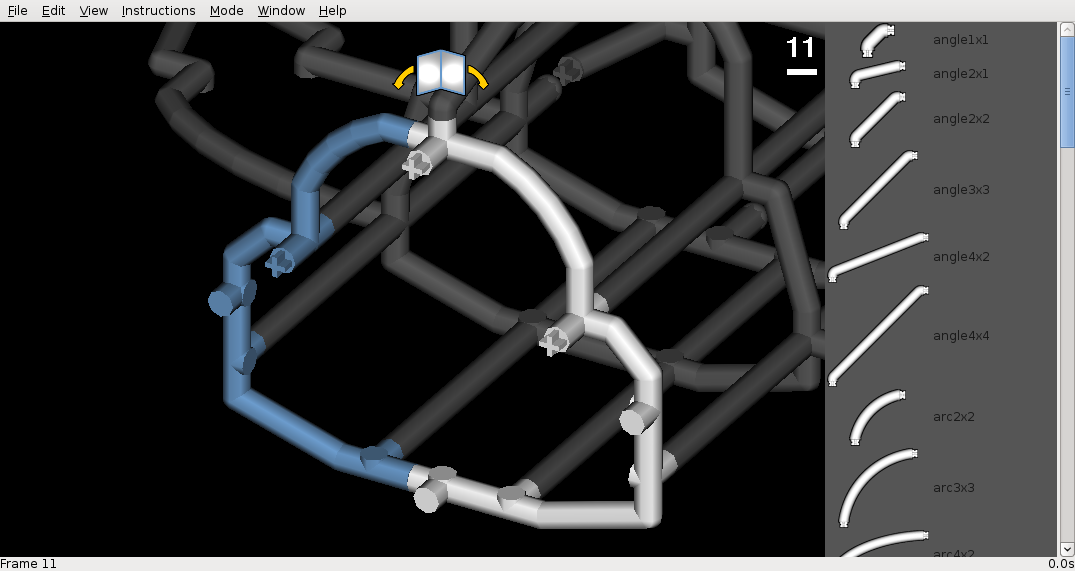
\includegraphics[width=5.38in]{doc_images/manual_instructions_mirror.png}
\caption{Mirror}
\label{InstructionsMirror}
\end{center}
\end{figure}

Many models are symmetric.  You can easily create a symmetric side
without many additional frames in your instruction set.  Use {\tt
  Instructions - Show Mirror} to display a mirror icon in your current
frame.  Drag the icon with the left mouse button to a position on the
frame's top between the symmetric sides.  Then, select all symmetric
pieces (Figure \ref{InstructionsMirror}).  By convention, hide the
part labels when mirroring by using {\tt Instructions - Hide Part
  Labels}.  Modellers should know a symmetric section uses the same
pieces.

Sometimes, models are repetitive.  For example, the body of a rocket
copies itself a number of times.  Following the same mirror
convention, you may use the mirror icon as a copying symbol too.

\subsection{Submodels}

\begin{figure}[H]
\begin{center}
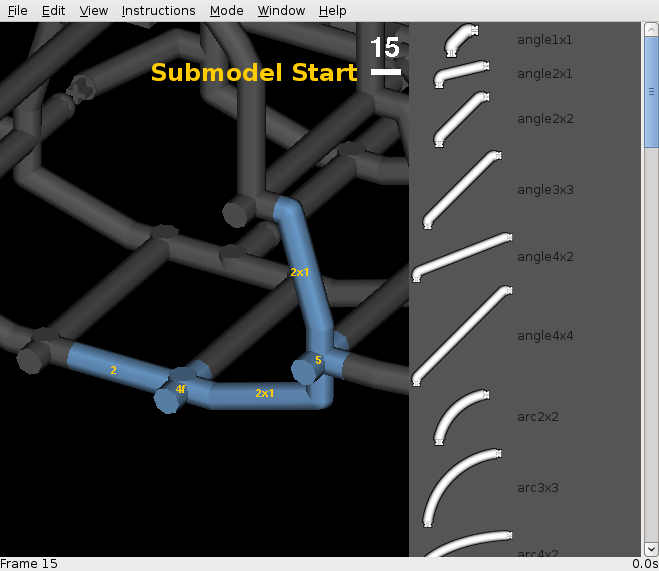
\includegraphics[width=3.29in]{doc_images/manual_instructions_submodel_start.png}
\caption{Submodel Start}
\label{InstructionsSubmodelStart}
\end{center}
\end{figure}

\begin{figure}[h]
\begin{center}
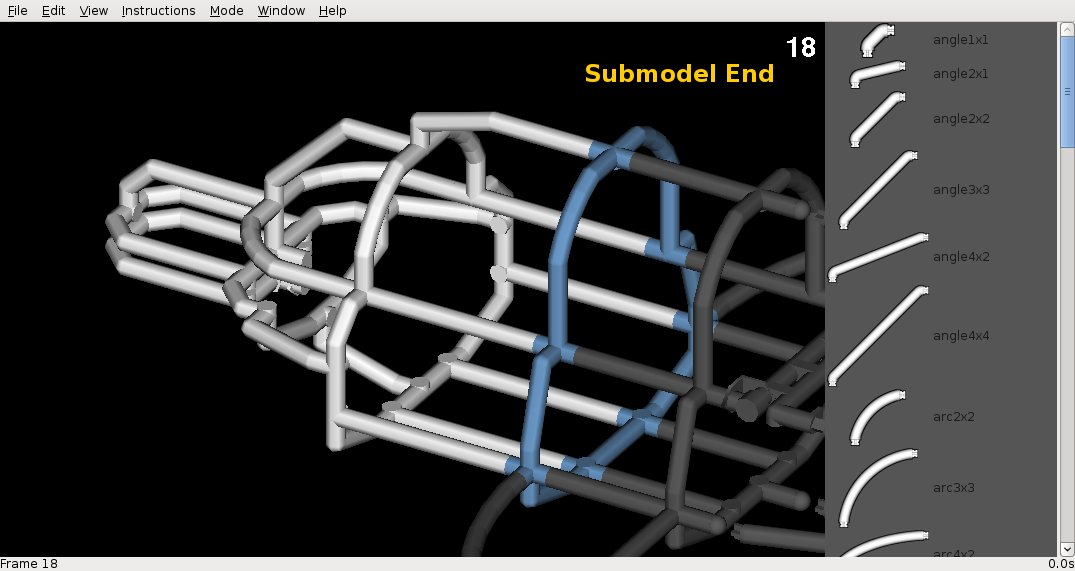
\includegraphics[width=5.38in]{doc_images/manual_instructions_submodel_end.png}
\caption{Submodel End}
\label{InstructionsSubmodelEnd}
\end{center}
\end{figure}

Sometimes it can be convenient or necessary to create a separate small
model (a submodel) that later attaches to the main model.  To begin a
submodel, select the {\tt Instructions - Start Submodel} menu option.
You'll notice the previous frame's white pieces disapper and a bar
beneath the frame number (Figure \ref{InstructionsSubmodelStart}).
The number of bars indicate the submodel depth.  No bars indicate the
main model.

Create the submodel the same way you create a main model: choose
window size, navigate, select pieces, navigate, and advance each frame
until you complete the submodel.  Once you complete the submodel
advance to the next frame, then use {\tt Instructions - End Submodel}.
You'll see the submodel in blue attached to the main model (Figure
\ref{InstructionsSubmodelEnd}).  Then, advance to the next frame and
you may proceed with main model frame creation.

The Crossbeams Modeller currently allows any depth of submodelling,
but watch out.  Submodelling causes confusion.

\subsection{Conventions}

\begin{figure}[h]
\begin{minipage}[t]{0.5\textwidth}
\begin{center}
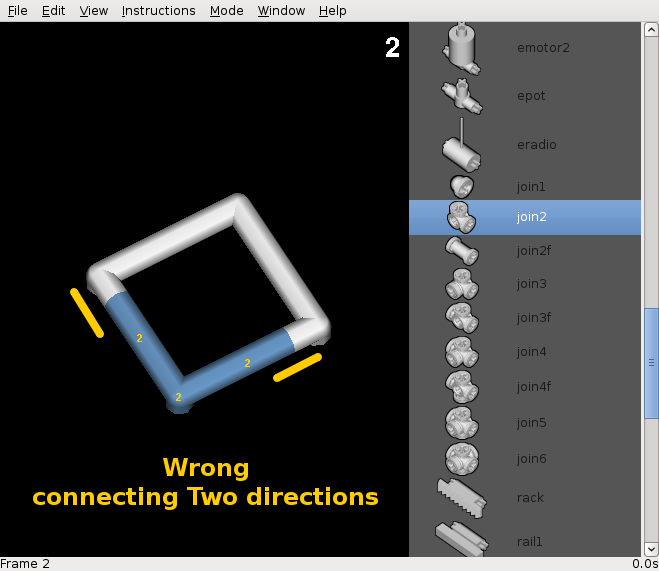
\includegraphics[width=3.125in]{doc_images/manual_instructions_loop_wrong.png}
\caption{Wrong Loop Connection}
\label{InstructionsLoopWrong}
\end{center}
\end{minipage}
\begin{minipage}[t]{0.5\textwidth}
\begin{center}
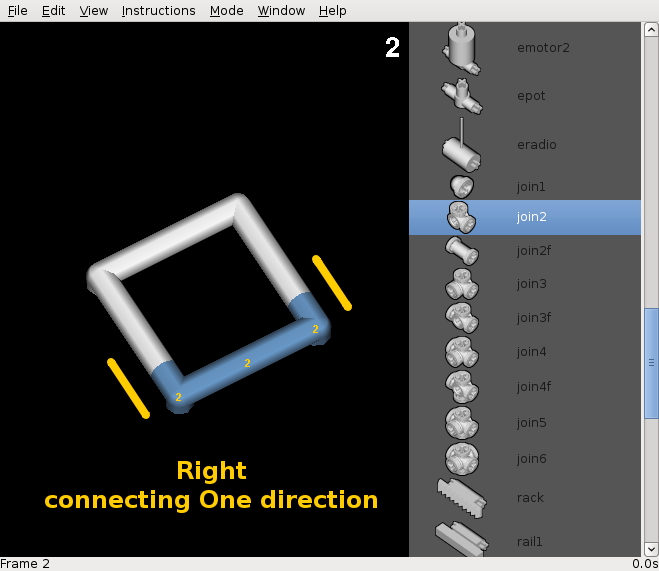
\includegraphics[width=3.125in]{doc_images/manual_instructions_loop_right.png}
\caption{Right Loop Connection}
\label{InstructionsLoopRight}
\end{center}
\end{minipage}
\end{figure}

When connecting loops (a connected set of pieces that close on
itself), the order of piece connection is important.  For example, you
should not create a square by adding one piece at a time.  Instead,
you should create two square halves and attach the halves together to
avoid straining the pieces (Figures \ref{InstructionsLoopWrong} and
\ref{InstructionsLoopRight}).  Make sure all new pieces in a frame can
be assembled to each other one piece at a time.  Then, make sure the
new pieces can attach to the old pieces without strain.

Zoom-in to a point where the part labels are distinguishable.  Use
Half and Full pages when the location of your added pieces may not be
clear.  Every few frames zoom out so the context is clear.

Use keyboard navigation for orbitting.  Preferably, begin with an
orthogonal view, go two steps right (or left), and two steps up (or
down).  Panning may be done with the mouse or keyboard.

Do not use partial zooms (the zooms arrived at by holding {\tt
  Control}).  Use only {\tt +} or {\tt -} levels of zooming.

Models with 250 pieces or less are beginner models.  Do not use
mirrors.  Try to hold to at most one submodel depth.  Add at most 5
pieces per frame.

Models with 250 to 750 pieces are intermediate models.  You may use
mirrors and any submodel depth.  Except for mirrors, add at most 7
pieces per frame.  Always Hide Part Labels when using mirrors.  Try to
minimize submodel depth.

Models with more than 750 pieces are advanced models.  You may use
mirrors and any submodel depth.  You may add as many pieces as you
want per frame; however, keep the instructions clear.  Always Hide
Part Labels when using mirrors.  Try to minimize submodel depth.

To create a good-looking instruction set, ask yourself the following
questions after every frame:

\begin{itemize}

  \item Have I closed loops from one direction only?

  \item Do the shown pieces take up most of the frame?

  \item Have I used large frames periodically to clearly know the
  position in the full model I'm currently working?

  \item Have I used keyboard poses and zooms?

  \item Do I have any labels overlapping?

  \item Do any labels go off the screen?

  \item Does my choice of frame sizes avoid blank frame space?

  \item Have I kept submodel depth minimum?

\end{itemize}

Many Crossbeams models are generated for a variety of skill levels.
We suggest the following skill levels and naming conventions.

\begin{center}
\begin{tabular}{ccc}
Level & Number of Pieces & Filename Suffix\\
\hline
1 & up to 220 & \_l1\\
2 & 200-450 & \_l2\\
3 & 400-650 & \_l3\\
4 & 600-1300 & \_l4\\
5 & 1000 or more & \_l5\\
\end{tabular}
\end{center}

\subsection{Generating a PDF}

Use {\tt Instructions - Generate} to generate a {\tt .pdf} form of
your instructions for sharing or printing.  Document generation takes
a while; you can watch progress in the \emph{Status Bar}.  The {\tt
  .pdf} file is placed in the same directory as your model.  It does
not \emph{pop up} when done.

Instructions are usually generated in \emph{Draft} mode, a 100
dots-per-inch (dpi) mode.  Higher resolution 300dpi instructions can
be achieved by unchecking {\tt Instructions - Draft}.  Watch out,
though.  High resolution instructions take longer to generate.
Additionally, high resolution windows usually go off screen.  Some
graphics cards don't generate off-screen images, and you'll get junk.
Start the Crossbeams Modeller using the {\tt -i} or {\tt --indirect}
option to guarantee proper off-screen instruction generation.  Of
course, indirect rendering is slower than direct rendering.

Some {\tt .pdf} viewers filelock the {\tt .pdf}.  In that case, close
the old {\tt .pdf} before generating a new {\tt .pdf} or use a viewer
that doesn't filelock.

\section{Nuances}

The screen shots in this document show a {\tt Windows} menu.  It was
renamed the {\tt Options} menu, which better describes its content.

All software has bugs, and new software has new bugs.  Losing your
work can be frustrating.  Save early, save often, and save revisions.

\section{Customization}

\subsection{Key Commands}

Where logical, key commands are similar to Blender.  The default
keyboard commands follow.

\begin{center}
\begin{longtable}{lp{2.5in}l}
Key & Command & Python Call \\
\hline
\endhead
p & Align the next part port with the model & \verb toggle_port() \\
Shift p & Align the previous part port with the model & \verb toggle_port(-1) \\
f & Rotate the part $90 ^\circ$ & \verb flip_port() \\
Shift f & Rotate the part $-90 ^\circ$ & \verb flip_port() \\
c & Connect the part to the model & \verb connect_part() \\
g & Grab and move selected parts & \verb grab() \\
Shift d & Duplicate selected parts & \verb duplicate() \\
r & Rotate selected parts & \verb rotate() \\
Control m & Mirror selected parts & \verb mirror() \\
b & Border select & \verb border_select() \\
a & Deselect all parts or select all parts & \verb select_all() \\
x & Delete selected parts & \verb delete_part() \\
Control z & Undo the last model change & \verb undo() \\
Controy y & Redo the last undo & \verb redo() \\
F2 & Write model (same as File -- Save As) & \verb write_file() \\
F1 & Read model (same as File -- Open) & \verb read_file() \\
z & Solid Detail (same as View -- Detail -- Solid) & \verb solid() \\
F12 & Render Detail (same as View -- Detail -- Render) & \verb render() \\
NumPad 7 & Top View & \verb viewstandard("top") \\
NumPad 1 & Front View & \verb viewstandard("front") \\
NumPad 3 & Right View & \verb viewstandard("right") \\
Shift NumPad 7 & Bottom View & \verb viewstandard("bottom") \\
Shift NumPad 1 & Back View & \verb viewstandard("back") \\
Shift NumPad 3 & Left View & \verb viewstandard("left") \\
NumPad 9 & Redraw the screen & \verb redraw_screen() \\
NumPad 8 & Orbit up & \verb orbitup() \\
NumPad 2 & Orbit down & \verb orbitdown() \\
NumPad 4 & Orbit left & \verb orbitleft() \\
NumPad 6 & Orbit right & \verb orbitright() \\
Shift NumPad 8 & Pan up & \verb panup() \\
Shift NumPad 2 & Pan down & \verb pandown() \\
Shift NumPad 4 & Pan left & \verb panleft() \\
Shift NumPad 6 & Pan right & \verb panright() \\
NumPad / & Rotate counter-clockwise & \verb rotateccw() \\
NumPad * & Rotate clockwise & \verb rotatecw() \\
NumPad + & Zoom in & \verb zoomin() \\
Control NumPad + & Zoom in 0.25x & \verb zoomin(0.25) \\
NumPad - & Zoom out & \verb zoomout() \\
Control NumPad - & Zoom out 0.25x & \verb zoomout(0.25) \\
Right Arrow & Next frame & \verb toggle_frame() \\
Left Arrow & Previous frame & \verb toggle_frame(None, -1) \\
Control q & Quit (same as File -- Quit) & \verb quit() \\
\label{PythonTable}
\end{longtable}
\end{center}

If you prefer a different key setup, edit (or create) a configuration
file.  For Linux and Mac users, the configuration file is {\tt
  .cbmodelrc} in {\tt HOME}, where {\tt HOME} is an environment
variable.  For Windows users, the configuration file is {\tt
  cbmodel.ini} in \verb USERPROFILE\AppData, where {\tt USERPROFILE}
is an environment variable.

\subsection{Configuration File}

The configuration file ({\tt .cbmodelrc} or {\tt cbmodel.ini})
contains user preferences.  Lines beginning with {\tt \#} (comments)
and blank lines are ignored.  Key settings can be changed in the {\tt
  [Keys]} section with {\tt function() = key}, where {\tt function()}
is the Python call and {\tt key} is the key name.  Start the
Crossbeams Modeller with the {\tt -p} or {\tt --printkeys} option to
see the key names in the \emph{Status Bar}.

An example configuration file follows:

\begin{verbatim}
# config file for users without a numeric keypad

[Keys]
redrawscreen() = o
orbitup() = i
panup() = <Shift>i
orbitdown() = comma
pandown() = <Shift>less
orbitleft() = j
panleft() = <Shift>j
orbitright() = l
panright() = <Shift>l
rotateccw() = 8
rotatecw() = 9

zoomin() = <Shift>plus
zoomin(0.25) = <Shift><Control>plus
zoomout() = minus
zoomout(0.25) = <Control>minus

viewstandard("top") = u
viewstandard("bottom") = <Shift>u
viewstandard("front") = m
viewstandard("back") = <Shift>m
viewstandard("right") = period
viewstandard("left") = <Shift>greater
\end{verbatim}

\end{document}
